One of the important concepts to understand when paralleling work is the two concepts of step and work complexity. Each of these two terms describe a different cost in term of the complexity it takes for an algorithm to be run. Step complexity is the concept of how many steps its going to take for a given algorithm, whereas work complexity is the amount of work it is going to take for the given algorithm to finish. \Cref{fig:stepnwork} displays an example where a given operation independent of ordering, such as plus of multiplication, is performed on eight elements in a three like structure. For this given example the work complexity would be seven(assuming that each of the seven operations have a work complexity of 1), as if we were to for instance add eight number together i would take seven plus operations. Meanwhile, as we divided our algorithm into a tree like structure, we have a step at each level of the tree, thereby giving a total of three steps.

\begin{figure}[ht]
	\centering
	\fbox{
		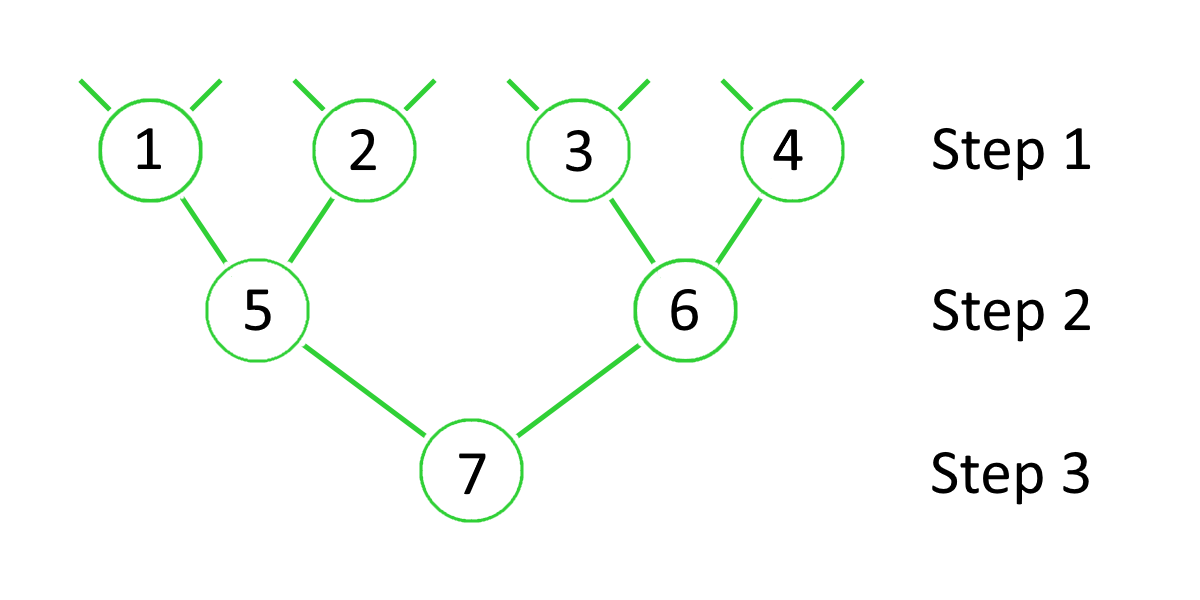
\includegraphics[width=0.6\textwidth]{figs/intro/step_work.png}
	}
	\caption{Step and work complexity example.}
	\label{fig:stepnwork}
\end{figure}

Step and work complexity is important in parallel programming, as we for a given algorithm, attempt to reduce the step complexity, thereby performing doing more in parallel at each step, by sacrificing work complexity. The idea behind this is that if the number of steps is reduced in our parallel implementation compared to our serial implementation, and work complexity is only slightly increased, our parallel algorithm will perform better then the serial algorithm.